\section{Results}

\subsection{Evaluation of Existing Models}
We evaluated the performance of IACA, llvm-mca, Ithemal\cite{ithemal}, and OSACA\cite{osaca}
on Haswell and Skylake.
We use relative error (i.e. absolute error of the predicted throughput normalized by the measured throughput)
as the metric to measure inaccuracy.
Table \ref{tab:overall} shows the unweighted average error
of each model on different microarchitectures.
% include ivb and skl
Figure \ref{fig:hsw-app-err, fig:skl-app-err} shows the breakdown of the errors by applications.
Figure \ref{fig:hsw-cluster-err, fig:skl-cluster-err} shows the breakdown of the errors by basic block clusters
(see \ref{classification} for details of basic blocks classification).

Ithemal\cite{ithemal} has the lowest overall error (12.53\%) on Haswell,
about 5\% better than the next best model, IACA.
The overall error of each model can however be unrepresentative
of its performance on a given domain.
For example, all the models we evaluated differ from
actual measurement by more than 30\% when evaluated on vectorized basic blocks.
The discrepancy between these models' overall unweighted accuracy
and that of specialized domains (e.g. numerical kernels) highlights
the need of basic block classification and per-class error reporting.

Generally speaking, basic blocks dominated by stores
(cluster-2, 3, and 20) are easier to predict,
while the throughput of basic blocks that mixes load instructions
with other operations (e.g. cluster-3 and cluster-7) are significantly 
more difficult to predict -- the prediction error is on average more than
twice higher than predicting basic blocks with only stores. 
We surmise that this is due to weakness of existing analyzers to model 
dynamic memory dependence.
In addition to basic blocks with memory dependence,
vectorized basic blocks (e.g. cluster-10) also causes high prediction errors.
% TODO: explain WHY vectorized basic blocks are hard to predict?

\begin{table}
\begin{tabular}{|p{0.25\columnwidth}|p{0.3\columnwidth}|p{0.3\columnwidth}|}
\hline

Microarchitecture & Model & Average Error\\
\hline

Haswell & IACA & 0.1798\\
    & llvm-mca & 0.1832\\
    & Ithemal & 0.1253\\
    & OSACA & 0.3916\\
    
\hline 
Skylake & IACA & 0.1578\\
    & llvm-mca & 0.2278\\
    & Ithemal & 0.4210\\
    & OSACA & 0.3768\\

\hline
% TODO more for IVB and SKL
\end{tabular}
\\
\caption{Overall error of evaluated models.}
\label{tab:overall}
\end{table}

\begin{figure}
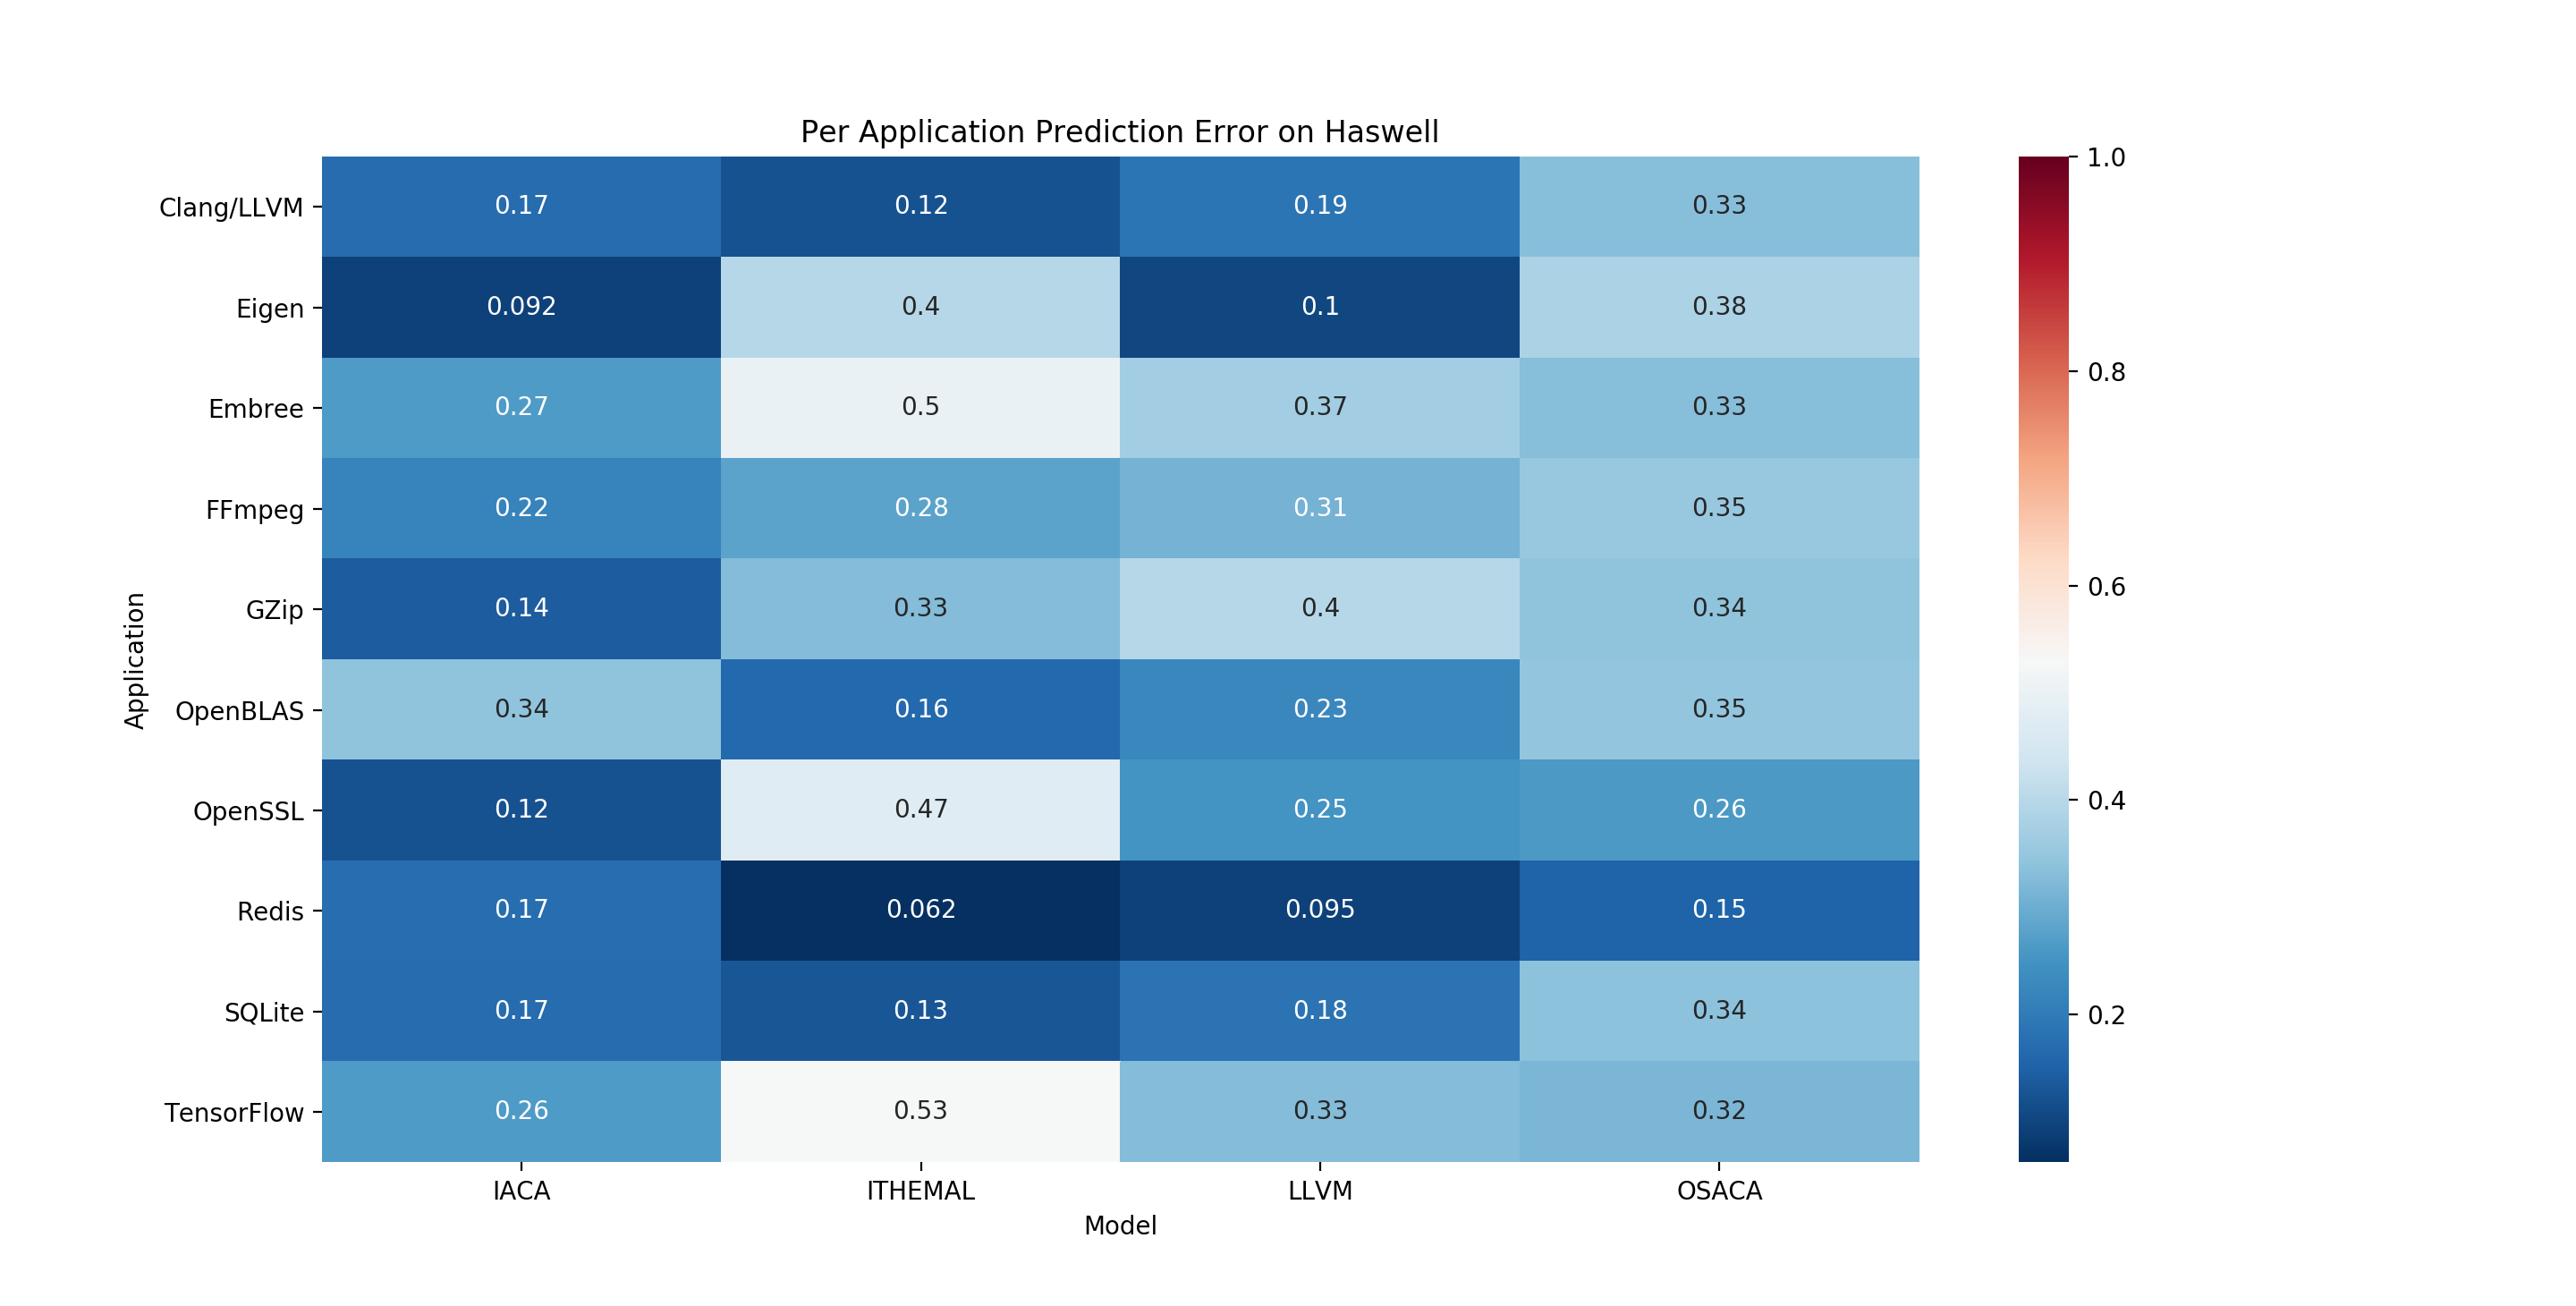
\includegraphics[width=\columnwidth]{figures/hsw-app-err.png}
\caption{Per-application error for each model on Haswell;
error for each basic block is weighted by the frequency it is sampled during profiling.}
\label{fig:hsw-app-err}
\end{figure}

\begin{figure}
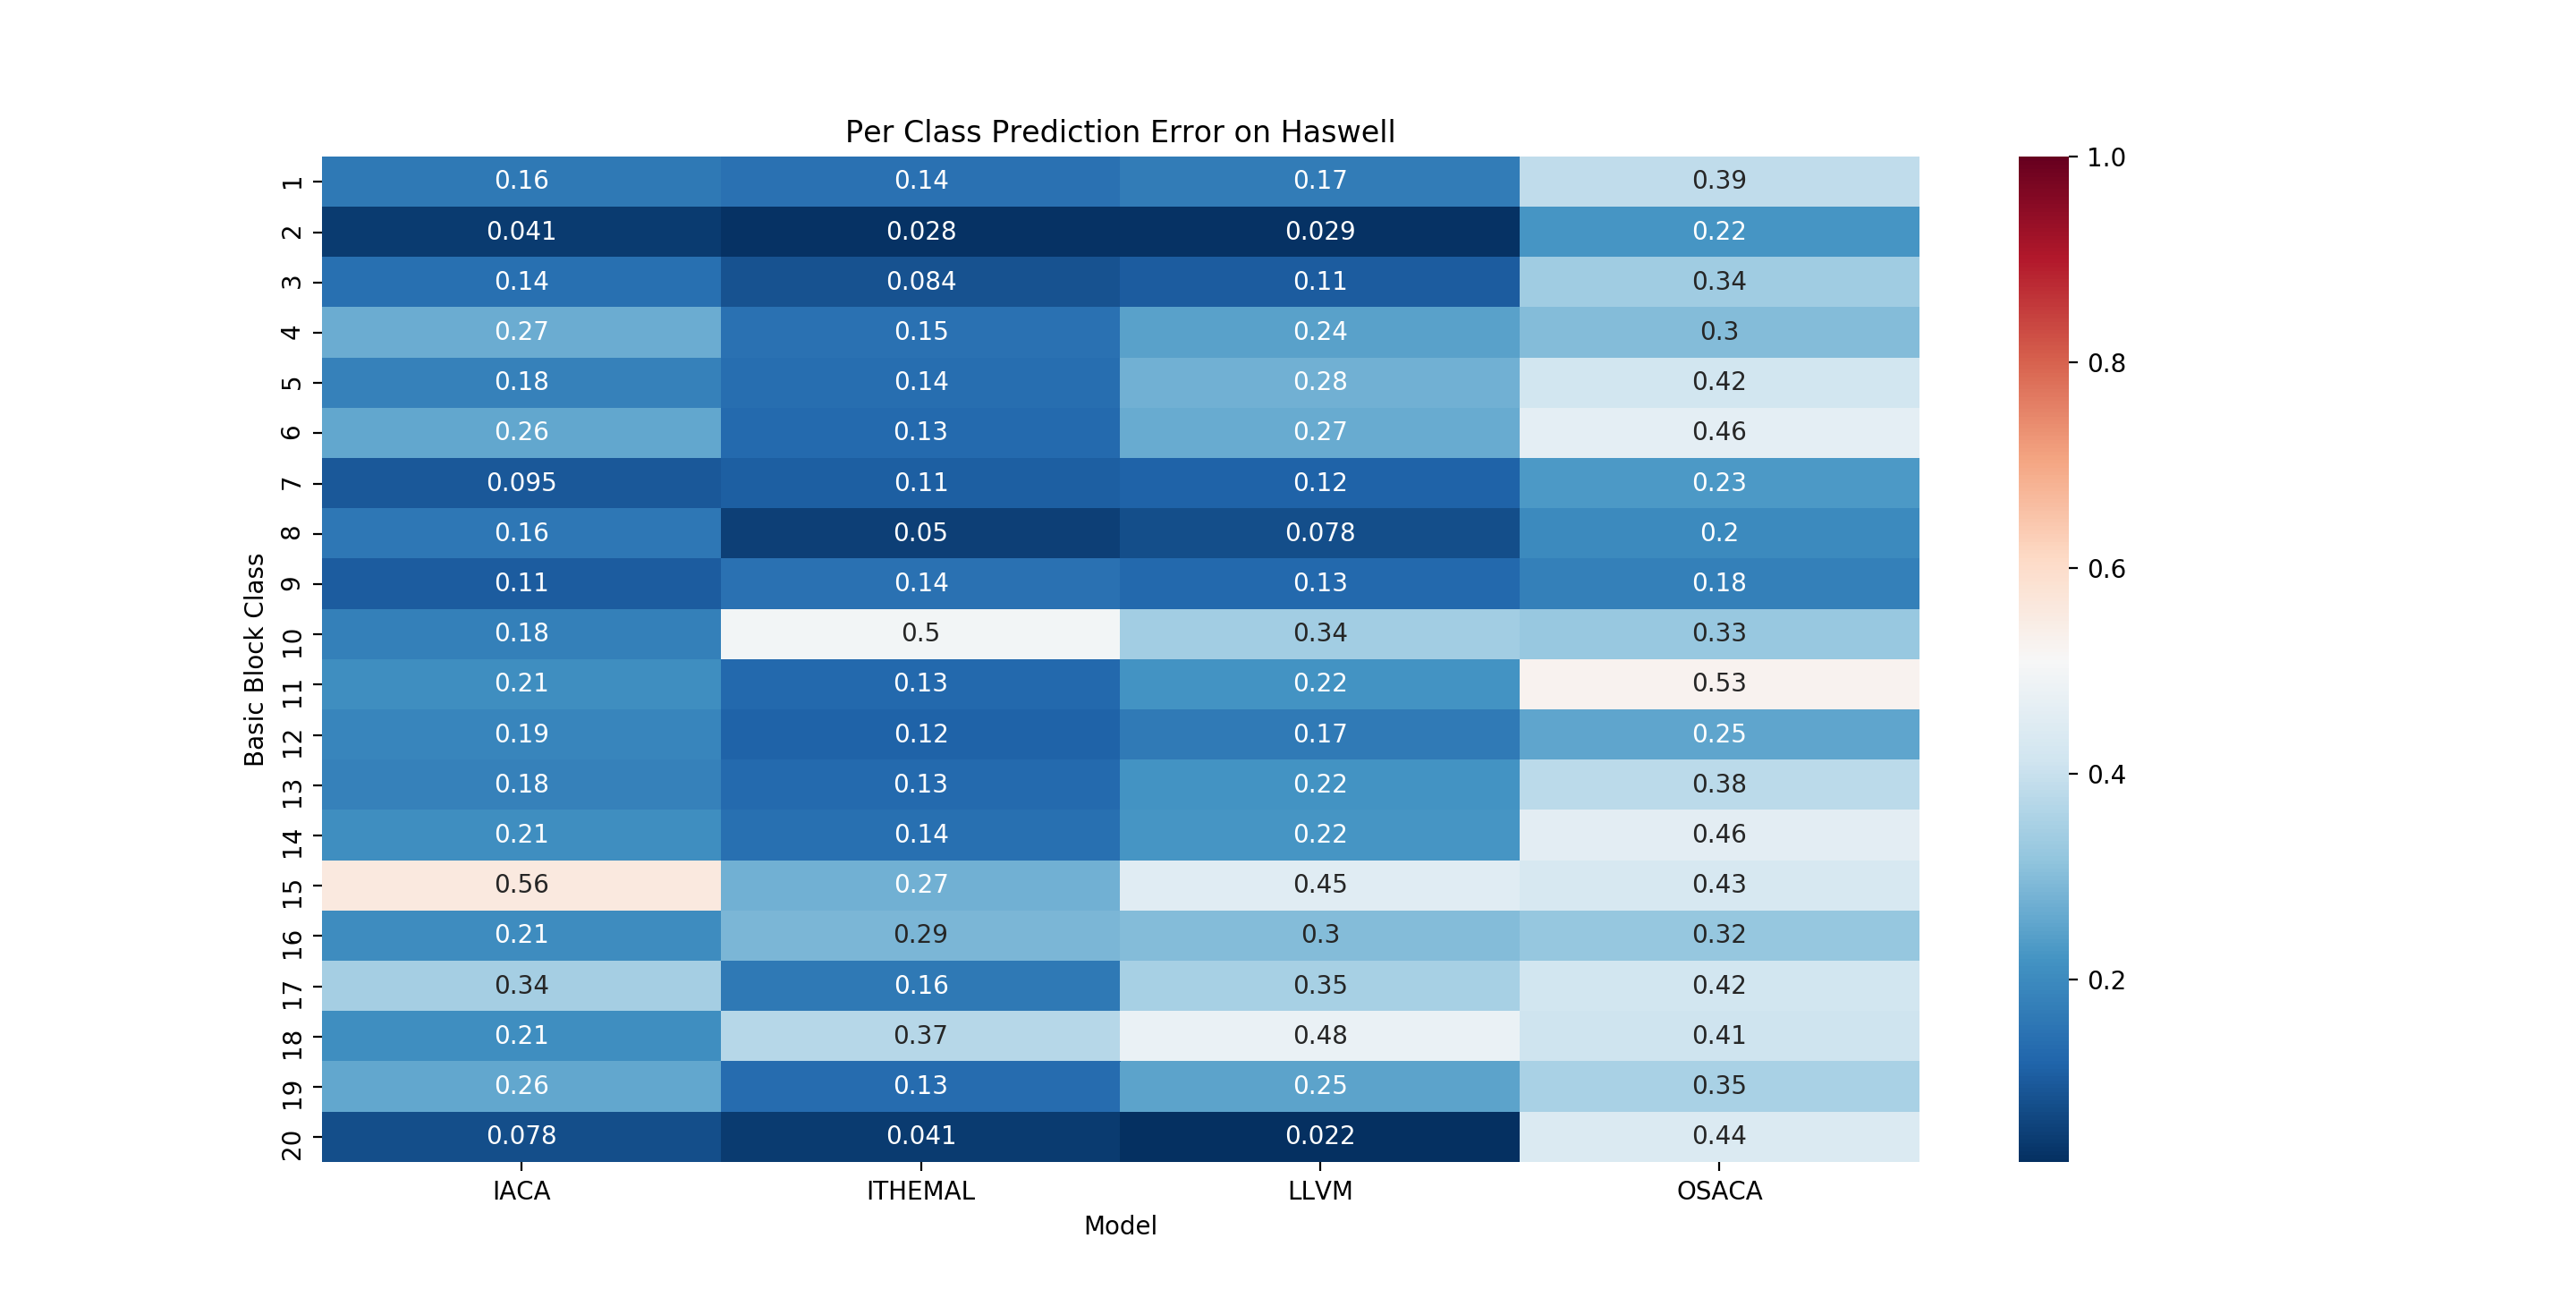
\includegraphics[width=\columnwidth]{figures/hsw-cluster-err.png}
\caption{Per-cluster error for each model on Haswell}
\label{fig:hsw-cluster-err}
\end{figure}

\begin{figure}
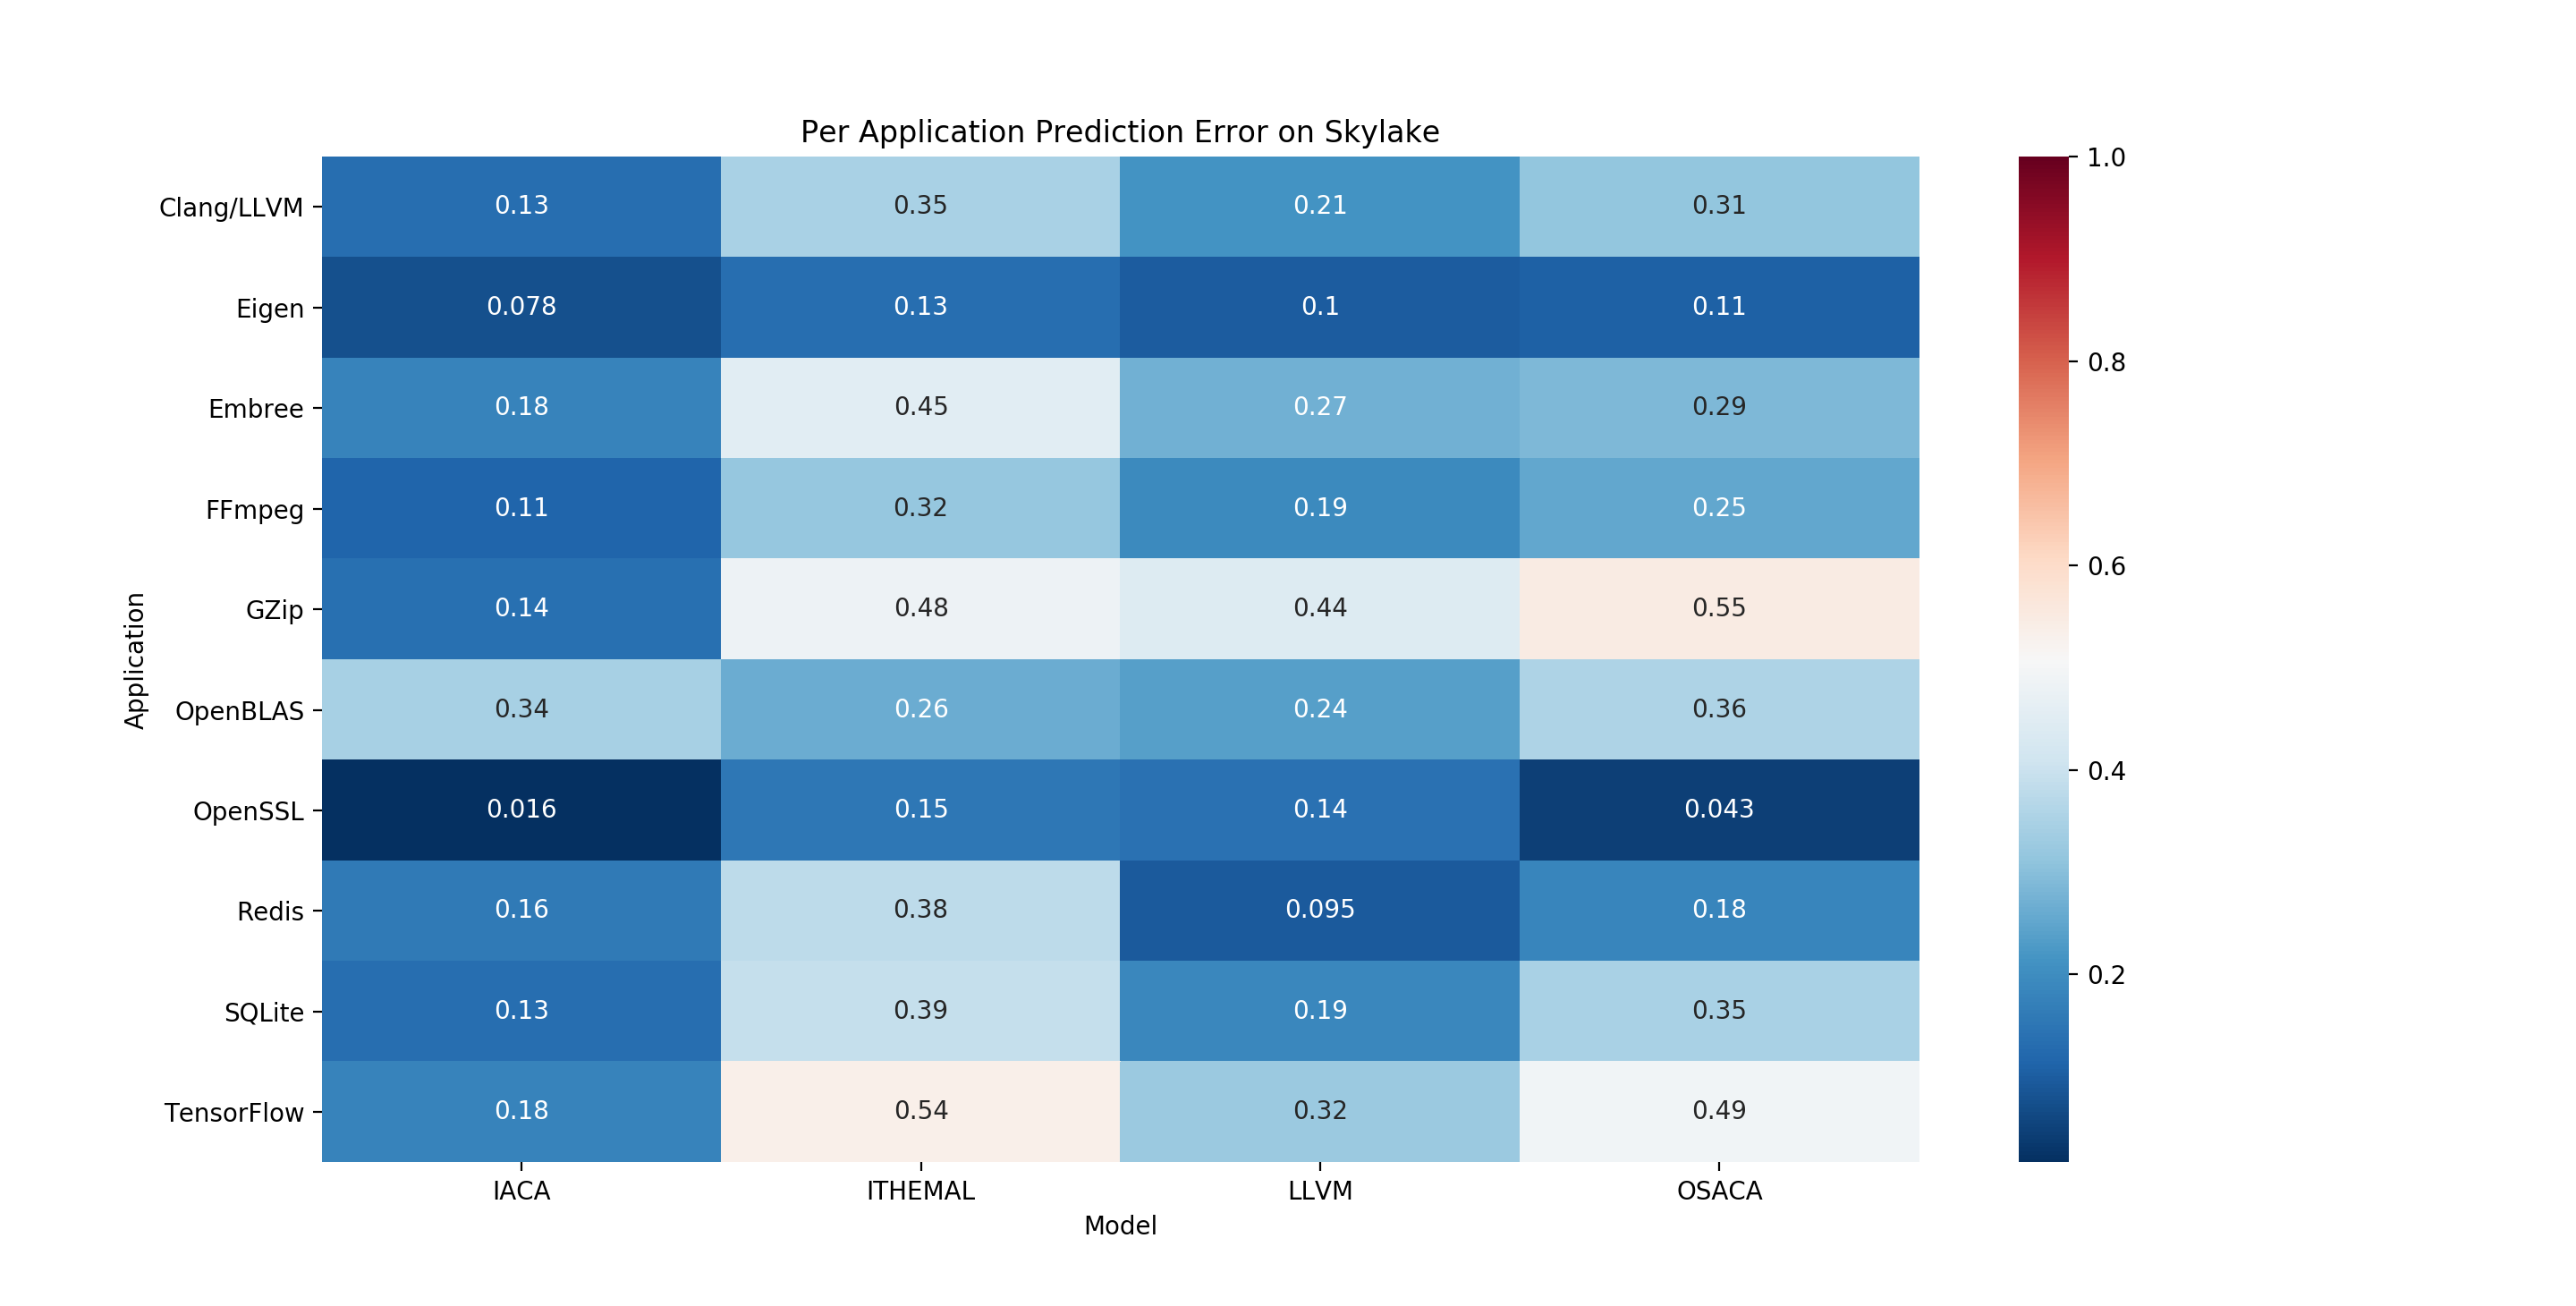
\includegraphics[width=\columnwidth]{figures/skl-app-err.png}
\caption{Per-application error for each model on Skylake. }
\label{fig:hsw-app-err}
\end{figure}

\begin{figure}
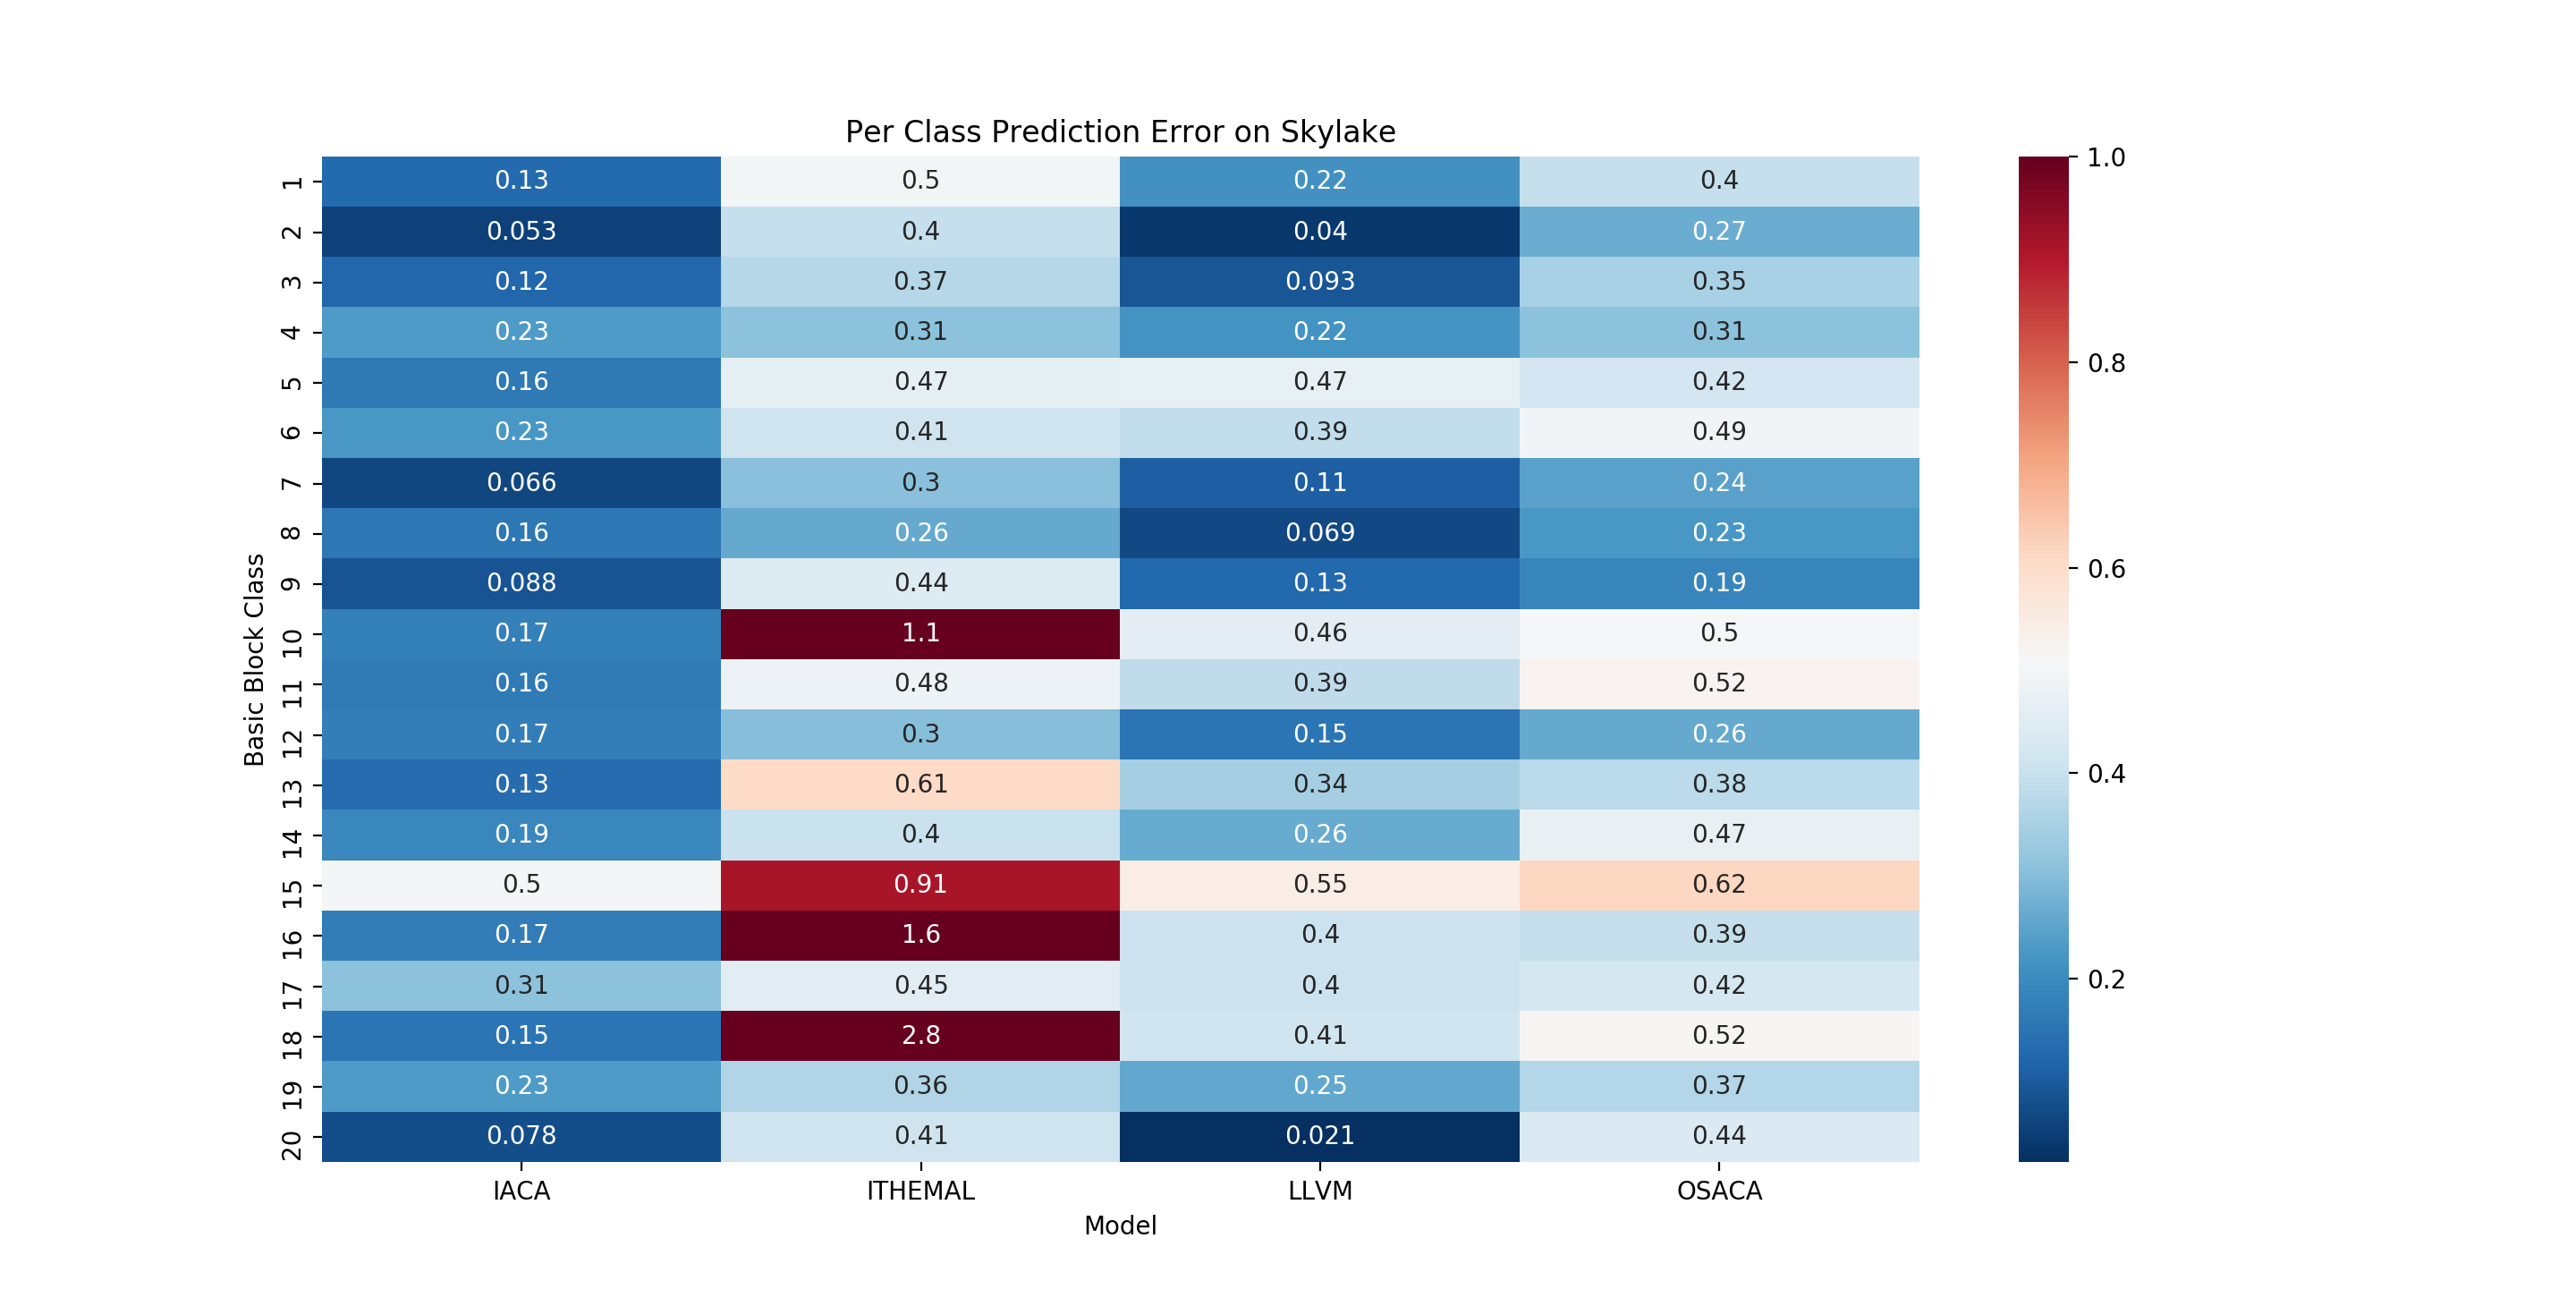
\includegraphics[width=\columnwidth]{figures/skl-cluster-err.png}
\caption{Per-cluster error for each model on Skylake}
\label{fig:hsw-cluster-err}
\end{figure}    
